%polyhedra beeldverwerking
\subsection{Beeldverwerking Polyhedra}
{\em Auteur: Laura Vranken}
\\
\\
% eerste stap: splitsen per kleur en binnen/buiten/obstakel
% tweede stap: voor elke kleur de buitenste acht randpunten zoeken
%			   dubbele eruit halen
% derde stap: alleen die overhouden die nog maar 3 hoekpunten hebben (half volledig)
% vierde stap: checken op zwaartepunt overeenkomt
% vijfde stap: linker en rechterbeeld samenvoegen om zwptn te krijgen voor xyz
\noindent
Om naar polyhedra te kunnen vliegen, moet de drone ze eerst kunnen herkennen op de ontvangen beelden. Het analyseren van de beelden gebeurt als volgt. 
\\
Ten eerste worden alle pixels gegroepeerd per kleur. Dan worden de kleuren opgesplitst in verschillende lijsten volgens hun soort, nl. binnen- en buitendriehoek van respectievelijk target en obstakel. Zie tabel \ref{table: HSVwaarden} voor de exacte voorwaarden.
\begin{table}[h]
	\centering
\begin{tabular}{ l | c | c | c }
	 & H & S & V\\\hline
	Buitendriehoek target & ? & \(>\) 0.55 & \(>\) 0.55 \\
	Binnendriehoek target & ? & \(<\) 0.45 & \(>\) 0.55 \\
	Buitendriehoek obstakel & ? & \(>\) 0.55 & \(<\) 0.45 \\
	Binnendriehoek obstakel & ? & \(<\) 0.45 & \(<\) 0.45\\
\end{tabular}
\caption{\label{table: HSVwaarden}Combinatie HSV-waarden om de verschillende driehoeken te herkennen. Hue waarde mag willekeurig gekozen worden.}
\end{table}
\\
Om het zwaartepunt van de driehoek te kunnen bepalen, wordt eerst naar de hoekpunten gezocht. Hiervoor wordt de buitenste pixel van elke zijde van de driehoek berekend. Aangezien het kan zijn dat twee hoekpunten op dezelfde lijn pixels liggen, worden twee pixels van elke zijde bepaald (de minimum en maximum pixel). Op deze manier worden acht pixels gevonden. Figuur \ref{fig:DrieGevallenDriehoeken}a geeft een voorbeeld van deze methode. Natuurlijk heeft een driehoek geen acht hoeken, dus worden de overeenkomstige buitenste pixels samengenomen tot één hoekpunt. 
\\\\
Een volledige driehoek behoudt drie hoekpunten. Ook kan een driehoek die evenwijdig met een zijde door een andere polyhedra of door de rand van het beeld afgesneden wordt, drie hoekpunten overhouden. Indien niet evenwijdig met een zijde wordt afgesneden, blijven er vier of meer hoekpunten over. Zie Figuur \ref{fig:DrieGevallenDriehoeken}b voor het eerste geval en Figuur \ref{fig:DrieGevallenDriehoeken}c voor het tweede geval. De figuren met meer dan drie hoekpunten worden niet meer bekeken; ze zijn niet volledig.
\\\\
Om onderscheid te maken tussen volledige en afgesneden driehoeken met drie hoekpunten, wordt de buitendriehoek samen met de overeenkomstige binnendriehoek verder onderzocht. Indien hun zwaartepunten samenvallen, zijn ze volledig. Indien ze niet matchen, kan geconcludeerd worden dat een deel van de driehoek is weggevallen. Zwaartepunten kunnen bepaald worden door Formule \ref{formule: zwaartepunt}: \begin{equation}
\label{formule: zwaartepunt}
(x_{zpt},y_{zpt}) = ( \ \frac{1}{3}(x_1 + x_2 + x_3) , \ \frac{1}{3}(y_1 + y_2 + y_3) \ )
\end{equation}
\\
Dit gebeurt voor beide camera's en vervolgens worden de gevonden zwaartepunten gecombineerd en doorgestuurd naar de fysische component van de Autopilot om omgezet te worden naar 3D-co\"ordinaten in het wereldassenstelsel. Uit deze re\"ele punten zal de dichtstbijzijnde polyhedron gevonden worden en als doel ingesteld worden.
\\
\begin{figure}[h]
	\centering
	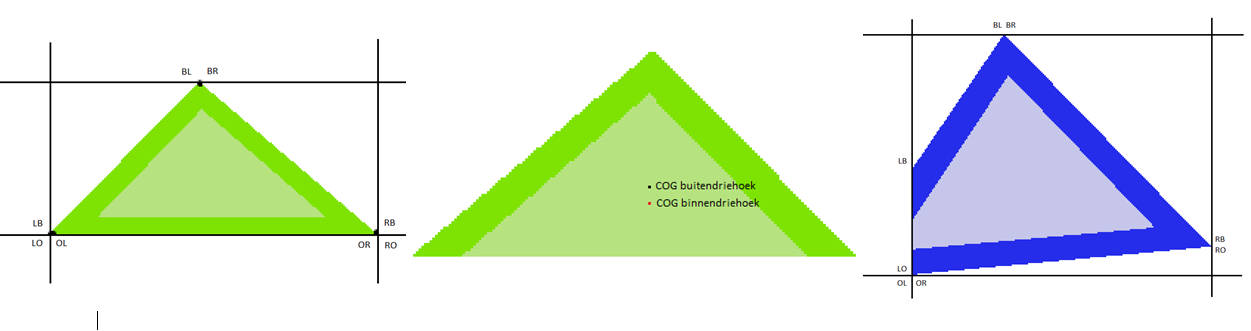
\includegraphics[width=1\textwidth]{BeeldverwerkingDriehoeken.png}
	\caption{Bepalen van de buitenste 8 punten van mogelijke driehoeken. \\ a) Een volledige driehoek. \\ b) Evenwijdig afgesneden driehoek met 3 hoekpunten. De zwaartepunten (COG) liggen echter op een andere plaats. \\ c) Willekeurig afgesneden driehoek met vier hoekpunten. \\ 
	Afkortingen: LO = links onder, LB = links boven, RO = rechts onder, RB = rechts boven, OL = onder links, OR = onder rechts, BL = boven links, BR = boven rechts.}
	\label{fig:DrieGevallenDriehoeken}
\end{figure}

